\begin{frame}{$d(K^-, p)"\pi^-\Lambda"$ 断面積 { \bf (Run68) }}
  \label{page:pimL_CS}
  
  \begin{figure}
    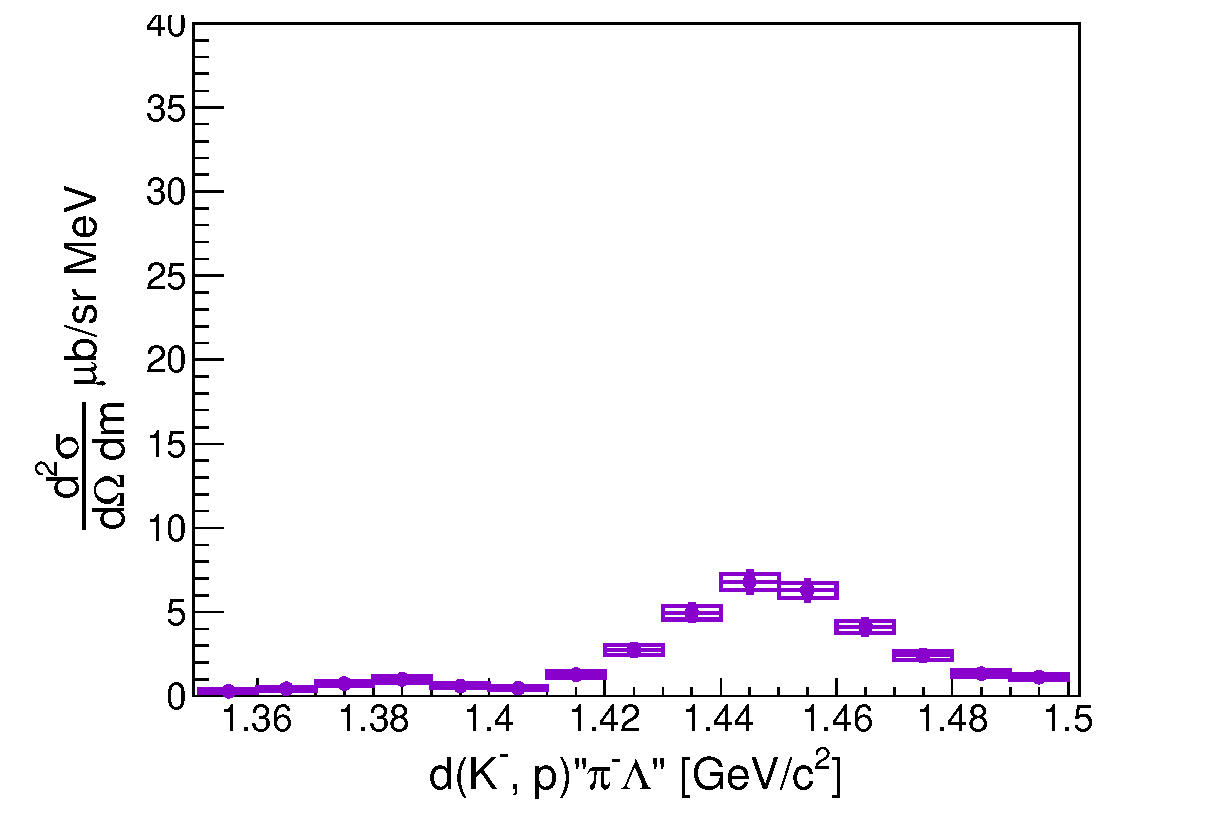
\includegraphics[width=8cm]{../pic/Run68/KP_ana/pimL_CS.eps}
  \end{figure}
  \centering
  トリガーの効率は取り込み済み\\
  標的の密度は改定済み\\
\end{frame}
